%-----------------------------------------------------------------------------------------------------------------------------------------------%
%	The MIT License (MIT)
%
%	Copyright (c) 2019 Jan Küster
%
%	Permission is hereby granted, free of charge, to any person obtaining a copy
%	of this software and associated documentation files (the "Software"), to deal
%	in the Software without restriction, including without limitation the rights
%	to use, copy, modify, merge, publish, distribute, sublicense, and/or sell
%	copies of the Software, and to permit persons to whom the Software is
%	furnished to do so, subject to the following conditions:
%	
%	THE SOFTWARE IS PROVIDED "AS IS", WITHOUT WARRANTY OF ANY KIND, EXPRESS OR
%	IMPLIED, INCLUDING BUT NOT LIMITED TO THE WARRANTIES OF MERCHANTABILITY,
%	FITNESS FOR A PARTICULAR PURPOSE AND NONINFRINGEMENT. IN NO EVENT SHALL THE
%	AUTHORS OR COPYRIGHT HOLDERS BE LIABLE FOR ANY CLAIM, DAMAGES OR OTHER
%	LIABILITY, WHETHER IN AN ACTION OF CONTRACT, TORT OR OTHERWISE, ARISING FROM,
%	OUT OF OR IN CONNECTION WITH THE SOFTWARE OR THE USE OR OTHER DEALINGS IN
%	THE SOFTWARE.
%	
%
%-----------------------------------------------------------------------------------------------------------------------------------------------%


%============================================================================%
%
%	DOCUMENT DEFINITION
%
%============================================================================%

%we use article class because we want to fully customize the page and don't use a cv template
\documentclass[10pt,A4]{article}	


%----------------------------------------------------------------------------------------
%	ENCODING
%----------------------------------------------------------------------------------------

% we use utf8 since we want to build from any machine
\usepackage[utf8]{inputenc}		

%----------------------------------------------------------------------------------------
%	LOGIC
%----------------------------------------------------------------------------------------

% provides \isempty test
\usepackage{xstring, xifthen}

%----------------------------------------------------------------------------------------
%	FONT BASICS
%----------------------------------------------------------------------------------------

% some tex-live fonts - choose your own

%\usepackage[defaultsans]{droidsans}
%\usepackage[default]{comfortaa}
%\usepackage{cmbright}
\usepackage[default]{raleway}
%\usepackage{fetamont}
%\usepackage[default]{gillius}
%\usepackage[light,math]{iwona}
%\usepackage[thin]{roboto} 

% set font default
\renewcommand*\familydefault{\sfdefault} 	
\usepackage[T1]{fontenc}

% more font size definitions
\usepackage{moresize}

%----------------------------------------------------------------------------------------
%	FONT AWESOME ICONS
%---------------------------------------------------------------------------------------- 

% include the fontawesome icon set
\usepackage{fontawesome}

% use to vertically center content
% credits to: http://tex.stackexchange.com/questions/7219/how-to-vertically-center-two-images-next-to-each-other
\newcommand{\vcenteredinclude}[1]{\begingroup
\setbox0=\hbox{\includegraphics{#1}}%
\parbox{\wd0}{\box0}\endgroup}

% use to vertically center content
% credits to: http://tex.stackexchange.com/questions/7219/how-to-vertically-center-two-images-next-to-each-other
\newcommand*{\vcenteredhbox}[1]{\begingroup
\setbox0=\hbox{#1}\parbox{\wd0}{\box0}\endgroup}

% icon shortcut
\newcommand{\icon}[3] { 							
	\makebox(#2, #2){\textcolor{darkcol}{\csname fa#1\endcsname}}
}	

% icon with text shortcut
\newcommand{\icontext}[4]{ 						
	\vcenteredhbox{\icon{#1}{#2}{#3}}  \hspace{2pt}  \parbox{0.9\mpwidth}{\textcolor{#4}{#3}}
}

% icon with website url
\newcommand{\iconhref}[5]{ 						
    \vcenteredhbox{\icon{#1}{#2}{#5}}  \hspace{2pt} \href{#4}{\textcolor{#5}{#3}}
}

% icon with email link
\newcommand{\iconemail}[5]{ 						
    \vcenteredhbox{\icon{#1}{#2}{#5}}  \hspace{2pt} \parbox{0.9\mpwidth}{\href{mailto:#4}{\textcolor{#5}{#3}}}
}

%----------------------------------------------------------------------------------------
%	PAGE LAYOUT  DEFINITIONS
%----------------------------------------------------------------------------------------

% page outer frames (debug-only)
% \usepackage{showframe}		

% we use paracol to display breakable two columns
\usepackage{paracol}

% define page styles using geometry
\usepackage[a4paper]{geometry}

% remove all possible margins
\geometry{top=1cm, bottom=1cm, left=1cm, right=1cm}

\usepackage{fancyhdr}
\pagestyle{empty}

% space between header and content
% \setlength{\headheight}{0pt}

% indentation is zero
\setlength{\parindent}{0mm}

%----------------------------------------------------------------------------------------
%	TABLE /ARRAY DEFINITIONS
%---------------------------------------------------------------------------------------- 

% extended aligning of tabular cells
\usepackage{array}

% custom column right-align with fixed width
% use like p{size} but via x{size}
\newcolumntype{x}[1]{%
>{\raggedleft\hspace{0pt}}p{#1}}%


%----------------------------------------------------------------------------------------
%	GRAPHICS DEFINITIONS
%---------------------------------------------------------------------------------------- 

%for header image
\usepackage{graphicx}

% use this for floating figures
% \usepackage{wrapfig}
% \usepackage{float}
% \floatstyle{boxed} 
% \restylefloat{figure}

%for drawing graphics		
\usepackage{tikz}				
\usetikzlibrary{shapes, backgrounds,mindmap, trees}

%----------------------------------------------------------------------------------------
%	Color DEFINITIONS
%---------------------------------------------------------------------------------------- 
\usepackage{transparent}
\usepackage{color}

% primary color
\definecolor{maincol}{RGB}{ 225, 0, 0 }

% accent color, secondary
 \definecolor{accentcol}{RGB}{ 10, 160, 250 }

% dark color
\definecolor{darkcol}{RGB}{ 1, 90, 153 }

% light color
\definecolor{lightcol}{RGB}{245,245,245}


% Package for links, must be the last package used
\usepackage[hidelinks]{hyperref}

% returns minipage width minus two times \fboxsep
% to keep padding included in width calculations
% can also be used for other boxes / environments
\newcommand{\mpwidth}{\linewidth-\fboxsep-\fboxsep}
	


%============================================================================%
%
%	CV COMMANDS
%
%============================================================================%

%----------------------------------------------------------------------------------------
%	 CV LIST
%----------------------------------------------------------------------------------------

% renders a standard latex list but abstracts away the environment definition (begin/end)
\newcommand{\cvlist}[1] {
	\begin{itemize}{#1}\end{itemize}
}

%----------------------------------------------------------------------------------------
%	 CV TEXT
%----------------------------------------------------------------------------------------

% base class to wrap any text based stuff here. Renders like a paragraph.
% Allows complex commands to be passed, too.
% param 1: *any
\newcommand{\cvtext}[1] {
	\begin{tabular*}{1\mpwidth}{p{0.98\mpwidth}}
		\parbox{1\mpwidth}{#1}
	\end{tabular*}
}

%----------------------------------------------------------------------------------------
%	CV SECTION
%----------------------------------------------------------------------------------------

% Renders a a CV section headline with a nice underline in main color.
% param 1: section title
\newcommand{\cvsection}[1] {
	\vspace{14pt}
	\cvtext{
		\textbf{\LARGE{\textcolor{darkcol}{\uppercase{#1}}}}\\[-4pt]
		\textcolor{accentcol}{ \rule{0.1\textwidth}{2pt} } \\
	}
}

%----------------------------------------------------------------------------------------
%	META SKILL
%----------------------------------------------------------------------------------------

% Renders a progress-bar to indicate a certain skill in percent.
% param 1: name of the skill / tech / etc.
% param 2: level (for example in years)
% param 3: percent, values range from 0 to 1
\newcommand{\cvskill}[3] {
	\begin{tabular*}{1\mpwidth}{p{0.72\mpwidth}  r}
 		\textcolor{black}{\textbf{#1}} & \textcolor{accentcol}{#2}\\
	\end{tabular*}%
	
	\hspace{4pt}
	\begin{tikzpicture}[scale=1,rounded corners=2pt,very thin]
		\fill [lightcol] (0,0) rectangle (1\mpwidth, 0.15);
		\fill [darkcol] (0,0) rectangle (#3\mpwidth, 0.15);
  	\end{tikzpicture}%
}


%----------------------------------------------------------------------------------------
%	 CV EVENT
%----------------------------------------------------------------------------------------

% Renders a table and a paragraph (cvtext) wrapped in a parbox (to ensure minimum content
% is glued together when a pagebreak appears).
% Additional Information can be passed in text or list form (or other environments).
% the work you did
% param 1: time-frame i.e. Sep 14 - Jan 15 etc.
% param 2:	 event name (job position etc.)
% param 3: Customer, Employer, Industry
% param 4: Short description
% param 5: work done (optional)
% param 6: technologies include (optional)
% param 7: achievements (optional)
\newcommand{\cvevent}[7] {
	
	% we wrap this part in a parbox, so title and description are not separated on a pagebreak
	% if you need more control on page breaks, remove the parbox
	\parbox{\mpwidth}{
		\begin{tabular*}{1\mpwidth}{p{0.72\mpwidth}  r}
	 		\textcolor{black}{\textbf{#2}} & \colorbox{darkcol}{\makebox[0.27\mpwidth]{\textcolor{white}{#1}}} \\
			\textcolor{darkcol}{\textbf{#3}} & \\
		\end{tabular*}\\[8pt]
	
		\ifthenelse{\isempty{#4}}{}{
			\cvtext{#4}\\
		}
	}

	\ifthenelse{\isempty{#5}}{}{
		\vspace{9pt}
		{#5}
	}

	\ifthenelse{\isempty{#6}}{}{
		\vspace{9pt}
		\cvtext{\textbf{Technologies include:}}\\
		{#6}
	}

	\ifthenelse{\isempty{#7}}{}{
		\vspace{9pt}
		\cvtext{\textbf{Achievements include:}}\\
		{#7}
	}
	\vspace{14pt}
}

%----------------------------------------------------------------------------------------
%	 CV META EVENT
%----------------------------------------------------------------------------------------

% Renders a CV event on the sidebar
% param 1: title
% param 2: subtitle (optional)
% param 3: customer, employer, etc,. (optional)
% param 4: info text (optional)
\newcommand{\cvmetaevent}[4] {
	\textcolor{maincol} {\cvtext{\textbf{\begin{flushleft}#1\end{flushleft}}}}

	\ifthenelse{\isempty{#2}}{}{
	\textcolor{darkcol} {\cvtext{\textbf{#2}} }
	}

	\ifthenelse{\isempty{#3}}{}{
		\cvtext{{ \textcolor{darkcol} {#3} }}\\
	}

	\cvtext{#4}\\[14pt]
}

%----------------------------------------------------------------------------------------
%	 CV contact event
%----------------------------------------------------------------------------------------

% Renders a CV event on the sidebar
% param 1: title
% param 2: subtitle (optional)
% param 3: customer, employer, etc,. (optional)
% param 4: info text (optional)
\newcommand{\cvcontactevent}[4] {
	\textcolor{maincol} {\cvtext{\textbf{\begin{flushleft}#1\end{flushleft}}}}

	\ifthenelse{\isempty{#2}}{}{
	\textcolor{darkcol} {\cvtext{\textbf{#2}} }
	}

	\ifthenelse{\isempty{#3}}{}{
		\cvtext{{ \textcolor{darkcol} {#3} }}\\
	}

	\cvtext{#4}\\[14pt]
}

%---------------------------------------------------------------------------------------
%	QR CODE
%----------------------------------------------------------------------------------------

% Renders a qrcode image (centered, relative to the parentwidth)
% param 1: percent width, from 0 to 1
\newcommand{\cvqrcode}[1] {
	\begin{center}
		
\includegraphics[width={#1}\mpwidth]{contact_qr.png}
	\end{center}
}


%============================================================================%
%
%
%
%	DOCUMENT CONTENT
%
%
%
%============================================================================%
\begin{document}
\columnratio{0.8}
\setlength{\columnsep}{2.2em}
\setlength{\columnseprule}{4pt}
\colseprulecolor{lightcol}
\begin{paracol}{2}
\begin{leftcolumn}

%---------------------------------------------------------------------------------------
%	TITLE  HEADER
%----------------------------------------------------------------------------------------
\fcolorbox{white}{darkcol}{\begin{minipage}[c][2.5cm][c]{1\mpwidth}
	\begin {center}
		\HUGE{ \textbf{ \textcolor{white}{ \uppercase{ Kevin Schmidiger } } } } \\[-24pt]
		\textcolor{white}{ \rule{0.1\textwidth}{1.25pt} } \\[4pt]
		\large{ \textcolor{white} {Software Engineer} }
	\end {center}
\end{minipage}} \\[14pt]
\vspace{-12pt}

\begin{minipage}[c][2.75cm][c]{1\mpwidth}
    \centering

   \parbox[c][2.5cm][c]{0.75\textwidth}{
   \centering
    \textbf{\textcolor{darkcol}{Die Wartbarkeit und Testbarkeit eines Programmes ist automatisch gegeben durch Clean Code.\\Sich mit neusten Technologien zu beschäftigen und an ihnen zu wachsen ist meine grösste Motivation.}}
}
\end{minipage}

\cvsection{Arbeitserfahrung}

\cvevent
	{Jun. 2022 - Heute}
	{ICT Applikationsentwickler}
	{\href{https://www.spsglobal.com/}{SPS Switzerland AG} - Papiergebundener Zahlungsvekehr}
	{\textbf{Aufgabengebiet:}
 \begin{itemize}
 \setlength\itemsep{-0.5em}
  \item Zuständig für sämtliche Applikationen im Zahlungsverkehr.
  \item Implementation von Features und Bugfixes.
  \item Vorantreiben des CI/CD Paradigma mit dem DevOps-Prozess als Ziel.
  \item Refactoring und Modernisierung (Upgrades der Java und C++ Versionen) der Legacy Applikationen.
\end{itemize}
\\\textbf{Technologien:}\\Java (ab 7), Java Servlet, HTML(/CSS), JavaScript, C/C++, SQL, Microsoft SQL Server/Windows, OLEDB, ProcMon, OCR, Git, Bash/Cmd scripting}
	{}
        {}
        {}

\begin{minipage}[c][0.5cm][c]{1\mpwidth}
%fill space
\end{minipage}

\cvevent
	{Jan. 2020 - Sept. 2021}
	{Senior Software Engineer}
	{\href{https://www.ssi-schaefer.com/}{SSI Schäfer AG} - Intralogistik}
	{\textbf{Aufgabengebiet:}
 \begin{itemize}
 \setlength\itemsep{-0.5em}
  \item Technischer Lead im Projektmanagent Team.
  \item Konzepterstellung und Machbarkeitsanalysen von Kundenlogistikprozessen in \href{https://www.ssi-schaefer.com/de-ch/software-loesungen/software-produkte/logistiksoftware-wamas--429726}{WAMAS} (\underline{Wa}rehouse \underline{Ma}nagement \underline{S}ystem, firmeneigene Logistiksoftware) in der DACH-Region.
  \item Erfassung und/oder ausarbeiten von Kundenanforderungen.
  \item Zuständig für den Aufbau und Weitergabe von Know-How.
  \item Vorhergehende Aufgaben.
\end{itemize}
\\\textbf{Technologien:}\\Java (7, 8, 11), Eclipse (IDE, RCP, RAP), RMI, RPC, JMS, REST, OSGi, SQL, Hibernate, SDC, BDeploy, Git, Gerrit, Linux Red Hat, Bash scripting}
	{}
        {}
        {}

\begin{minipage}[c][0.5cm][c]{1\mpwidth}
%fill space
\end{minipage}

\cvevent
	{Jul. 2017 - Dez. 2019}
	{Software Engineer}
	{\href{https://www.ssi-schaefer.com/}{SSI Schäfer AG} - Intralogistik}
	{\textbf{Aufgabengebiet:}
 \begin{itemize}
 \setlength\itemsep{-0.5em}
  \item Umsetzung von Kundenanforderungen in \href{https://www.ssi-schaefer.com/de-ch/software-loesungen/software-produkte/logistiksoftware-wamas--429726}{WAMAS} (\underline{Wa}rehouse \underline{Ma}nagement \underline{S}ystem, firmeneigene Logistiksoftware) in der DACH-Region, sowie Testing und Bugfixing.
  \item Zuständig für die Einarbeitung neuer Mitarbeiter.
  \item Stellvertretender Teamleiter.
  \item Lehrlingsbetreuung im Bereich Applikationsentwicklung (u. a. Betreuung durch die individuelle Praktische Arbeit (IPA)).
\end{itemize}}
	{}
        {}
        {}

\newpage

\begin{minipage}[c][0.75cm][c]{1\mpwidth}
%fill space
\end{minipage}

\cvevent
	{Okt. 2016 - Apr. 2017}
	{Software Engineer (Praktikum)}
	{\href{https://www.avaloq.com/}{Avaloq Evolution AG} - Tools Innovation}
	{6 monatiges Praktikum in einem internationalem Umfeld. \\ \\ \textbf{Aufgabengebiet:}
 \begin{itemize}
 \setlength\itemsep{-0.5em}
  \item Mitarbeit im  agilen Team der Tools Innovation (Eclipse Plug-ins).
  \item Entwicklung eines Plugins, um SQL-Abfragen in Eclipse abzusetzen.
  \item Kleinere Bugfixes und Features, sowie Testing.
\end{itemize}
\\\textbf{Technologien:}\\Java (7), Eclipse (IDE), OSGi, SQL, Git, Gerrit, SonarQube, Bash scripting}
    {}
    {}
    {}

\begin{minipage}[c][1cm][c]{1\mpwidth}
%fill space
\end{minipage}

\cvsection{Ausbildung}

\cvevent
	{2013 - 2018}
	{Bachelor of Science FHO in Informatik}
	{\href{http://www.hsr.ch/}{HSR Hochschule für Technik Rapperswil}}
	{\textbf{Bachelorarbeit}: \href{https://eprints.ost.ch/id/eprint/522/}{(Eclipse) Plug-in} für \href{https://isocpp.github.io/CppCoreGuidelines/CppCoreGuidelines}{C++ Core Guideline unterstüztung}\\
Einhaltung der Rules im Kapitel: \href{https://isocpp.github.io/CppCoreGuidelines/CppCoreGuidelines#S-ctor}{C.ctor: Constructors, assignments, and destructors} mithilfe von Codeanalyse und Refactoring}
	{}
        {}
        {}

\cvevent
	{2012 - 2013}
	{Berufsmaturität (Technische Richtung)}
	{\href{http://www.bbw.ch/}{BBW Berufsbildungsschule Winterthur}}
	{\textbf{Interdisziplinäre Projektarbeit (IDPA):} Spezielle Zahlen und Verhältnisse als Schönheit der Natur}
	{}
        {}
        {}

\cvevent
	{2007 - 2011}
	{Berufslehre Elektroinstallateur EFZ}
	{\href{htttp://www.tbz.ch/}{TBZ Technische Berufsschule Zürich}}
	{\textbf{Vertiefungsarbeit (VA):} 9/11 - Was ist wirklich passiert?}
	{}
        {}
        {}

\begin{minipage}[c][1cm][c]{1\mpwidth}
%fill space
\end{minipage}

\cvsection{Freizeit}

\begin{minipage}[c][4cm][c]{1\mpwidth}
\centering
   \parbox[c][2cm][c]{0.97\textwidth}{
    \textbf{Interessen}
    \begin{itemize}
 \setlength\itemsep{-0.5em}
  \item Laufen (bis und mit Streckenlänge Halbmarathon)
  \item Elektrotechnik (8-Bit Breadboard Computer gebaut, Kennenlernen vom\\ATmega328(p))
  \item Generative KI
  \item Programmiersprachen (Evolution von C++ und Java)
  \item Eishockey
  \item Astronomie
  \item generell technikinteressiert
\end{itemize}
}
\end{minipage}

% Insert stuff here

\end{leftcolumn}
\begin{rightcolumn}

%---------------------------------------------------------------------------------------
%	META IMAGE
%----------------------------------------------------------------------------------------
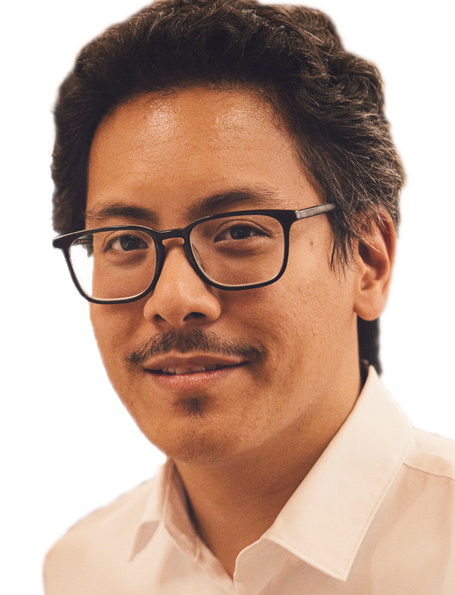
\includegraphics[width=\linewidth]{picture.png}	%trimming relative to image size

\cvsection{Kontakt}

\icontext{MapMarker}{12}{Konrad-Ilg-Str. 22\\8049 Zürich}{black}\\[6pt]
\icontext{MobilePhone}{12}{+41 79 269 82 25}{black}\\[6pt]
\iconemail{Envelope}{12}{schmidiger.kevin\\@hotmail.com}{schmidiger.kevin@hotmail.com}{black}\\[6pt]
\icontext{Calendar}{12}{02.12.1991}{black}\\[6pt]
%\cvqrcode{0.9} %from https://qrfy.com/my-qr-codes

\vfill

\cvsection{Skills}

\cvskill{Java} {8+ yrs} {1} \\[-2pt]

\cvskill{(C/)C++} {3+ yrs} {0.8} \\[-2pt]

\cvskill{SQL} {8+ yrs} {0.75} \\[-2pt]

\cvskill{HTML/CSS/JS} {2+ yrs} {0.6} \\[-2pt]

\vfill

\cvsection{Sprachen}

\cvskill{Deutsch\newline(Muttersprache)} {} {1} \\[-2pt]

\cvskill{English\newline(fliessend)} {} {0.8} \\[-2pt]

\vfill

% Insert stuff here

\end{rightcolumn}
\end{paracol}
\end{document}